% Generated by Sphinx.
\def\sphinxdocclass{report}
\documentclass[letterpaper,10pt,english]{sphinxmanual}
\usepackage[utf8]{inputenc}
\DeclareUnicodeCharacter{00A0}{\nobreakspace}
\usepackage{cmap}
\usepackage[T1]{fontenc}
\usepackage{babel}
\usepackage{times}
\usepackage[Bjarne]{fncychap}
\usepackage{longtable}
\usepackage{sphinx}
\usepackage{multirow}


\title{Application Exercises}
\date{January 14, 2015}
\release{0.1}
\author{Florian Genilloud}
\newcommand{\sphinxlogo}{}
\renewcommand{\releasename}{Release}
\makeindex

\makeatletter
\def\PYG@reset{\let\PYG@it=\relax \let\PYG@bf=\relax%
    \let\PYG@ul=\relax \let\PYG@tc=\relax%
    \let\PYG@bc=\relax \let\PYG@ff=\relax}
\def\PYG@tok#1{\csname PYG@tok@#1\endcsname}
\def\PYG@toks#1+{\ifx\relax#1\empty\else%
    \PYG@tok{#1}\expandafter\PYG@toks\fi}
\def\PYG@do#1{\PYG@bc{\PYG@tc{\PYG@ul{%
    \PYG@it{\PYG@bf{\PYG@ff{#1}}}}}}}
\def\PYG#1#2{\PYG@reset\PYG@toks#1+\relax+\PYG@do{#2}}

\expandafter\def\csname PYG@tok@gd\endcsname{\def\PYG@tc##1{\textcolor[rgb]{0.63,0.00,0.00}{##1}}}
\expandafter\def\csname PYG@tok@gu\endcsname{\let\PYG@bf=\textbf\def\PYG@tc##1{\textcolor[rgb]{0.50,0.00,0.50}{##1}}}
\expandafter\def\csname PYG@tok@gt\endcsname{\def\PYG@tc##1{\textcolor[rgb]{0.00,0.27,0.87}{##1}}}
\expandafter\def\csname PYG@tok@gs\endcsname{\let\PYG@bf=\textbf}
\expandafter\def\csname PYG@tok@gr\endcsname{\def\PYG@tc##1{\textcolor[rgb]{1.00,0.00,0.00}{##1}}}
\expandafter\def\csname PYG@tok@cm\endcsname{\let\PYG@it=\textit\def\PYG@tc##1{\textcolor[rgb]{0.25,0.50,0.56}{##1}}}
\expandafter\def\csname PYG@tok@vg\endcsname{\def\PYG@tc##1{\textcolor[rgb]{0.73,0.38,0.84}{##1}}}
\expandafter\def\csname PYG@tok@m\endcsname{\def\PYG@tc##1{\textcolor[rgb]{0.13,0.50,0.31}{##1}}}
\expandafter\def\csname PYG@tok@mh\endcsname{\def\PYG@tc##1{\textcolor[rgb]{0.13,0.50,0.31}{##1}}}
\expandafter\def\csname PYG@tok@cs\endcsname{\def\PYG@tc##1{\textcolor[rgb]{0.25,0.50,0.56}{##1}}\def\PYG@bc##1{\setlength{\fboxsep}{0pt}\colorbox[rgb]{1.00,0.94,0.94}{\strut ##1}}}
\expandafter\def\csname PYG@tok@ge\endcsname{\let\PYG@it=\textit}
\expandafter\def\csname PYG@tok@vc\endcsname{\def\PYG@tc##1{\textcolor[rgb]{0.73,0.38,0.84}{##1}}}
\expandafter\def\csname PYG@tok@il\endcsname{\def\PYG@tc##1{\textcolor[rgb]{0.13,0.50,0.31}{##1}}}
\expandafter\def\csname PYG@tok@go\endcsname{\def\PYG@tc##1{\textcolor[rgb]{0.20,0.20,0.20}{##1}}}
\expandafter\def\csname PYG@tok@cp\endcsname{\def\PYG@tc##1{\textcolor[rgb]{0.00,0.44,0.13}{##1}}}
\expandafter\def\csname PYG@tok@gi\endcsname{\def\PYG@tc##1{\textcolor[rgb]{0.00,0.63,0.00}{##1}}}
\expandafter\def\csname PYG@tok@gh\endcsname{\let\PYG@bf=\textbf\def\PYG@tc##1{\textcolor[rgb]{0.00,0.00,0.50}{##1}}}
\expandafter\def\csname PYG@tok@ni\endcsname{\let\PYG@bf=\textbf\def\PYG@tc##1{\textcolor[rgb]{0.84,0.33,0.22}{##1}}}
\expandafter\def\csname PYG@tok@nl\endcsname{\let\PYG@bf=\textbf\def\PYG@tc##1{\textcolor[rgb]{0.00,0.13,0.44}{##1}}}
\expandafter\def\csname PYG@tok@nn\endcsname{\let\PYG@bf=\textbf\def\PYG@tc##1{\textcolor[rgb]{0.05,0.52,0.71}{##1}}}
\expandafter\def\csname PYG@tok@no\endcsname{\def\PYG@tc##1{\textcolor[rgb]{0.38,0.68,0.84}{##1}}}
\expandafter\def\csname PYG@tok@na\endcsname{\def\PYG@tc##1{\textcolor[rgb]{0.25,0.44,0.63}{##1}}}
\expandafter\def\csname PYG@tok@nb\endcsname{\def\PYG@tc##1{\textcolor[rgb]{0.00,0.44,0.13}{##1}}}
\expandafter\def\csname PYG@tok@nc\endcsname{\let\PYG@bf=\textbf\def\PYG@tc##1{\textcolor[rgb]{0.05,0.52,0.71}{##1}}}
\expandafter\def\csname PYG@tok@nd\endcsname{\let\PYG@bf=\textbf\def\PYG@tc##1{\textcolor[rgb]{0.33,0.33,0.33}{##1}}}
\expandafter\def\csname PYG@tok@ne\endcsname{\def\PYG@tc##1{\textcolor[rgb]{0.00,0.44,0.13}{##1}}}
\expandafter\def\csname PYG@tok@nf\endcsname{\def\PYG@tc##1{\textcolor[rgb]{0.02,0.16,0.49}{##1}}}
\expandafter\def\csname PYG@tok@si\endcsname{\let\PYG@it=\textit\def\PYG@tc##1{\textcolor[rgb]{0.44,0.63,0.82}{##1}}}
\expandafter\def\csname PYG@tok@s2\endcsname{\def\PYG@tc##1{\textcolor[rgb]{0.25,0.44,0.63}{##1}}}
\expandafter\def\csname PYG@tok@vi\endcsname{\def\PYG@tc##1{\textcolor[rgb]{0.73,0.38,0.84}{##1}}}
\expandafter\def\csname PYG@tok@nt\endcsname{\let\PYG@bf=\textbf\def\PYG@tc##1{\textcolor[rgb]{0.02,0.16,0.45}{##1}}}
\expandafter\def\csname PYG@tok@nv\endcsname{\def\PYG@tc##1{\textcolor[rgb]{0.73,0.38,0.84}{##1}}}
\expandafter\def\csname PYG@tok@s1\endcsname{\def\PYG@tc##1{\textcolor[rgb]{0.25,0.44,0.63}{##1}}}
\expandafter\def\csname PYG@tok@gp\endcsname{\let\PYG@bf=\textbf\def\PYG@tc##1{\textcolor[rgb]{0.78,0.36,0.04}{##1}}}
\expandafter\def\csname PYG@tok@sh\endcsname{\def\PYG@tc##1{\textcolor[rgb]{0.25,0.44,0.63}{##1}}}
\expandafter\def\csname PYG@tok@ow\endcsname{\let\PYG@bf=\textbf\def\PYG@tc##1{\textcolor[rgb]{0.00,0.44,0.13}{##1}}}
\expandafter\def\csname PYG@tok@sx\endcsname{\def\PYG@tc##1{\textcolor[rgb]{0.78,0.36,0.04}{##1}}}
\expandafter\def\csname PYG@tok@bp\endcsname{\def\PYG@tc##1{\textcolor[rgb]{0.00,0.44,0.13}{##1}}}
\expandafter\def\csname PYG@tok@c1\endcsname{\let\PYG@it=\textit\def\PYG@tc##1{\textcolor[rgb]{0.25,0.50,0.56}{##1}}}
\expandafter\def\csname PYG@tok@kc\endcsname{\let\PYG@bf=\textbf\def\PYG@tc##1{\textcolor[rgb]{0.00,0.44,0.13}{##1}}}
\expandafter\def\csname PYG@tok@c\endcsname{\let\PYG@it=\textit\def\PYG@tc##1{\textcolor[rgb]{0.25,0.50,0.56}{##1}}}
\expandafter\def\csname PYG@tok@mf\endcsname{\def\PYG@tc##1{\textcolor[rgb]{0.13,0.50,0.31}{##1}}}
\expandafter\def\csname PYG@tok@err\endcsname{\def\PYG@bc##1{\setlength{\fboxsep}{0pt}\fcolorbox[rgb]{1.00,0.00,0.00}{1,1,1}{\strut ##1}}}
\expandafter\def\csname PYG@tok@kd\endcsname{\let\PYG@bf=\textbf\def\PYG@tc##1{\textcolor[rgb]{0.00,0.44,0.13}{##1}}}
\expandafter\def\csname PYG@tok@ss\endcsname{\def\PYG@tc##1{\textcolor[rgb]{0.32,0.47,0.09}{##1}}}
\expandafter\def\csname PYG@tok@sr\endcsname{\def\PYG@tc##1{\textcolor[rgb]{0.14,0.33,0.53}{##1}}}
\expandafter\def\csname PYG@tok@mo\endcsname{\def\PYG@tc##1{\textcolor[rgb]{0.13,0.50,0.31}{##1}}}
\expandafter\def\csname PYG@tok@mi\endcsname{\def\PYG@tc##1{\textcolor[rgb]{0.13,0.50,0.31}{##1}}}
\expandafter\def\csname PYG@tok@kn\endcsname{\let\PYG@bf=\textbf\def\PYG@tc##1{\textcolor[rgb]{0.00,0.44,0.13}{##1}}}
\expandafter\def\csname PYG@tok@o\endcsname{\def\PYG@tc##1{\textcolor[rgb]{0.40,0.40,0.40}{##1}}}
\expandafter\def\csname PYG@tok@kr\endcsname{\let\PYG@bf=\textbf\def\PYG@tc##1{\textcolor[rgb]{0.00,0.44,0.13}{##1}}}
\expandafter\def\csname PYG@tok@s\endcsname{\def\PYG@tc##1{\textcolor[rgb]{0.25,0.44,0.63}{##1}}}
\expandafter\def\csname PYG@tok@kp\endcsname{\def\PYG@tc##1{\textcolor[rgb]{0.00,0.44,0.13}{##1}}}
\expandafter\def\csname PYG@tok@w\endcsname{\def\PYG@tc##1{\textcolor[rgb]{0.73,0.73,0.73}{##1}}}
\expandafter\def\csname PYG@tok@kt\endcsname{\def\PYG@tc##1{\textcolor[rgb]{0.56,0.13,0.00}{##1}}}
\expandafter\def\csname PYG@tok@sc\endcsname{\def\PYG@tc##1{\textcolor[rgb]{0.25,0.44,0.63}{##1}}}
\expandafter\def\csname PYG@tok@sb\endcsname{\def\PYG@tc##1{\textcolor[rgb]{0.25,0.44,0.63}{##1}}}
\expandafter\def\csname PYG@tok@k\endcsname{\let\PYG@bf=\textbf\def\PYG@tc##1{\textcolor[rgb]{0.00,0.44,0.13}{##1}}}
\expandafter\def\csname PYG@tok@se\endcsname{\let\PYG@bf=\textbf\def\PYG@tc##1{\textcolor[rgb]{0.25,0.44,0.63}{##1}}}
\expandafter\def\csname PYG@tok@sd\endcsname{\let\PYG@it=\textit\def\PYG@tc##1{\textcolor[rgb]{0.25,0.44,0.63}{##1}}}

\def\PYGZbs{\char`\\}
\def\PYGZus{\char`\_}
\def\PYGZob{\char`\{}
\def\PYGZcb{\char`\}}
\def\PYGZca{\char`\^}
\def\PYGZam{\char`\&}
\def\PYGZlt{\char`\<}
\def\PYGZgt{\char`\>}
\def\PYGZsh{\char`\#}
\def\PYGZpc{\char`\%}
\def\PYGZdl{\char`\$}
\def\PYGZhy{\char`\-}
\def\PYGZsq{\char`\'}
\def\PYGZdq{\char`\"}
\def\PYGZti{\char`\~}
% for compatibility with earlier versions
\def\PYGZat{@}
\def\PYGZlb{[}
\def\PYGZrb{]}
\makeatother

\begin{document}

\maketitle
\tableofcontents
\phantomsection\label{index::doc}


Contenu:


\chapter{L'application exercice, c'est quoi ?}
\label{projet_debut:permettre-au-professeur-de-creer-un-exercice-et-a-un-eleve-de-le-resoudre}\label{projet_debut::doc}\label{projet_debut:l-application-exercice-c-est-quoi}

\section{Introduction}
\label{projet_debut:introduction}
Voici la documentation de l'application Exercice présente sur le site \href{https://webmath-thirteenfoil8.c9.io/exercises/}{suivant} . Celle-ci vous premettra de
pouvoir utiliser la partie création ainsi que la partie résolution des exercices de manière complète et détaillée. Cette application servira par la suite à un
professeur de pouvoir créer un exercice ( principalement de factorisation ou bien de calcul) et de pouvoir le mettre en ligne. Il suffira de donner le lien de
l'exercice à l'élève pour qu'il puisse le résoudre.

Cette application consiste en premier lieu à avoir un support internet sur lequel un élève du Csud pourrait s'entraîner en prévision de ses examens ou alors tout simplement
pour perfectionner ses capacités en mathématique dans le domaine de la factorisation et dans celui du calcul. Elle est essentielle au projet pour que les professeurs puissent
créer des exercices selon le besoin de leur élève et pour pouvoir analyser les erreurs que les élèves font par rapport à ceux-ci. Cela permet aussi à un élève de savoir où sont
ses difficultés et de savoir quelles sont les thèmes qu'il doit travailler. Django permet de pouvoir stocker les données créées par les
professeurs dans une base de données et de pouvoir récupérer celle-ci pour en faire des pages. Cela est exactement ce dont nous avons besoin pour cette application car le
professeur en question créé un exercice et la partie backend très développée de Django s'occupe de créer la page web contenant les données entrées précédemment.


\section{La collaboration dans le projet}
\label{projet_debut:la-collaboration-dans-le-projet}
Pour ce qui est de la collaboration avec les autres applications du projet, il faudrait au minimum que les fonctionnalités suivantes soit disponible:
\begin{itemize}
\item {} 
La collaboration avec le dashboard élève:
\begin{itemize}
\item {} 
L'élève doit pouvoir ajouter les liens des exercices qu'il a trouvé compliqués.

\item {} 
Il doit pouvoir avoir un Feedback des exercices qu'il a déjà fait.

\item {} 
Il doit pouvoir mettre les liens des exercices à faire pour les devoirs ou autres dans un dossier.

\end{itemize}

\item {} 
La collaboration avec le dashboard professeur :
\begin{itemize}
\item {} 
Le professeur doit pouvoir faire des dossiers avec les exercices qu'il a créés.

\item {} 
Il doit également pouvoir prendre des exercices d'autres professeurs pour les intégrer dans un dossier.

\end{itemize}

\item {} 
La collaboration avec les cours:
\begin{itemize}
\item {} 
Un cours doit pouvoir contenir les liens des exercices qui sont en rapport avec ceux-ci.

\item {} 
Il faudrait pouvoir faire un dossier dans le cours avec les corrigés des exercices faisant partis de celui-ci.

\end{itemize}

\item {} 
La collaboration avec les quiz:
\begin{itemize}
\item {} 
Il faudrait pouvoir mettre en relation un exercice ou bien un groupe d'exercices avec un ou plusieurs quiz ayant le même but pédagogique.

\end{itemize}

\end{itemize}


\section{Intégration de l'application}
\label{projet_debut:integration-de-l-application}
L'intégration de cette application au reste du projet ne devrait normalement pas poser trop de problèmes. La manière la plus simple de faire correspondre les exercices à des cours ou autres est
d'utiliser les liens des exercices pour pouvoir y accéder.


\section{Le template de base du site}
\label{projet_debut:le-template-de-base-du-site}
Pour ce qui est du Frontend, suite à une mise en commun avec Benoît Léo, le créateur de l'application quiz, nous nous sommes mis d'accord pour utiliser le même
template de base bootstrap ce trouvant \href{http://startbootstrap.com/template-overviews/shop-item/}{ici} .

Pour ce qui est de la barre latéral se trouvant à gauche des pages du site, il a fallu mettre des liens vers les différents template. Ceci se fait non pas en recopiant le lien
de la page web directement mais en utilisant une commande django simple qui permet, si il y a un changement d'url par la suite dans le fichier urls.py de faire automatiquement le changement
pour éviter les erreurs de redirection.

le code est le suivant :

\begin{Verbatim}[commandchars=\\\{\}]
\PYG{o}{\PYGZlt{}}\PYG{n}{div} \PYG{n}{class}\PYG{o}{=}\PYG{l+s}{\PYGZdq{}}\PYG{l+s}{list\PYGZhy{}group}\PYG{l+s}{\PYGZdq{}}\PYG{o}{\PYGZgt{}}
    \PYG{o}{\PYGZlt{}}\PYG{n}{a} \PYG{n}{href}\PYG{o}{=}\PYG{l+s}{\PYGZdq{}}\PYG{l+s}{\PYGZob{}}\PYG{l+s+si}{\PYGZpc{} u}\PYG{l+s}{rl }\PYG{l+s}{\PYGZsq{}}\PYG{l+s}{exercises:index}\PYG{l+s}{\PYGZsq{}}\PYG{l+s}{ }\PYG{l+s}{\PYGZpc{}}\PYG{l+s}{\PYGZcb{}}\PYG{l+s}{\PYGZdq{}} \PYG{n}{class}\PYG{o}{=}\PYG{l+s}{\PYGZdq{}}\PYG{l+s}{list\PYGZhy{}group\PYGZhy{}item \PYGZob{}}\PYG{l+s}{\PYGZpc{}}\PYG{l+s}{ block active\PYGZhy{}home }\PYG{l+s}{\PYGZpc{}}\PYG{l+s}{\PYGZcb{}}
    \PYG{n}{active}\PYG{p}{\PYGZob{}}\PYG{o}{\PYGZpc{}} \PYG{n}{endblock} \PYG{o}{\PYGZpc{}}\PYG{p}{\PYGZcb{}}\PYG{l+s}{\PYGZdq{}}\PYG{l+s}{\PYGZgt{}Accueil\PYGZlt{}/a\PYGZgt{}}
    \PYG{o}{\PYGZlt{}}\PYG{n}{a} \PYG{n}{href}\PYG{o}{=}\PYG{l+s}{\PYGZdq{}}\PYG{l+s}{\PYGZob{}}\PYG{l+s+si}{\PYGZpc{} u}\PYG{l+s}{rl }\PYG{l+s}{\PYGZsq{}}\PYG{l+s}{exercises:find}\PYG{l+s}{\PYGZsq{}}\PYG{l+s}{ }\PYG{l+s}{\PYGZpc{}}\PYG{l+s}{\PYGZcb{}}\PYG{l+s}{\PYGZdq{}} \PYG{n}{class}\PYG{o}{=}\PYG{l+s}{\PYGZdq{}}\PYG{l+s}{list\PYGZhy{}group\PYGZhy{}item \PYGZob{}}\PYG{l+s}{\PYGZpc{}}\PYG{l+s}{ block active\PYGZhy{}reso }\PYG{l+s}{\PYGZpc{}}\PYG{l+s}{\PYGZcb{}}
    \PYG{p}{\PYGZob{}}\PYG{o}{\PYGZpc{}} \PYG{n}{endblock} \PYG{o}{\PYGZpc{}}\PYG{p}{\PYGZcb{}}\PYG{l+s}{\PYGZdq{}}\PYG{l+s}{\PYGZgt{}Résoudre un exercice\PYGZlt{}/a\PYGZgt{}}
    \PYG{o}{\PYGZlt{}}\PYG{n}{a} \PYG{n}{href}\PYG{o}{=}\PYG{l+s}{\PYGZdq{}}\PYG{l+s}{\PYGZob{}}\PYG{l+s+si}{\PYGZpc{} u}\PYG{l+s}{rl }\PYG{l+s}{\PYGZsq{}}\PYG{l+s}{exercises:create}\PYG{l+s}{\PYGZsq{}}\PYG{l+s}{ }\PYG{l+s}{\PYGZpc{}}\PYG{l+s}{\PYGZcb{}}\PYG{l+s}{\PYGZdq{}} \PYG{n}{class}\PYG{o}{=}\PYG{l+s}{\PYGZdq{}}\PYG{l+s}{list\PYGZhy{}group\PYGZhy{}item \PYGZob{}}\PYG{l+s}{\PYGZpc{}}\PYG{l+s}{ block active\PYGZhy{}create }\PYG{l+s}{\PYGZpc{}}\PYG{l+s}{\PYGZcb{}}
    \PYG{p}{\PYGZob{}}\PYG{o}{\PYGZpc{}} \PYG{n}{endblock} \PYG{o}{\PYGZpc{}}\PYG{p}{\PYGZcb{}}\PYG{l+s}{\PYGZdq{}}\PYG{l+s}{\PYGZgt{}Création d}\PYG{l+s}{\PYGZsq{}}\PYG{l+s}{exercice\PYGZlt{}/a\PYGZgt{}}
\PYG{o}{\PYGZlt{}}\PYG{o}{/}\PYG{n}{div}\PYG{o}{\PYGZgt{}}
\end{Verbatim}

Comme vous pouvez le constater, un block \{\% block active \%\} a été ajouté à chaque lien. Ceci permet d'activer la classe ``list-group-item'' dans la page actuel.


\section{Les modèles}
\label{projet_debut:les-modeles}
Les modèles de l'application Exercice ne sont pas très nombreux. Ils servent surtout à la création et à la résolution des exercices. ( A compléter)


\chapter{Comment, où créer un exercice}
\label{create:comment-ou-creer-un-exercice}\label{create::doc}

\section{La page de création d'exercice}
\label{create:la-page-de-creation-d-exercice}
L'application exercice possède un onglet \href{https://webmath-thirteenfoil8.c9.io/exercises/create/}{création d'exercice} , présent sur le menu latéral permettant de renvoyer à la page de
création d'exercice.

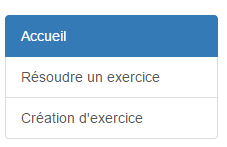
\includegraphics{onglet.png}

Cliquez sur l'onglet Création d'exercice pour aller sur la page de création. Une fois sur la page, un encadré ressemblant à ça devrait apparaître:

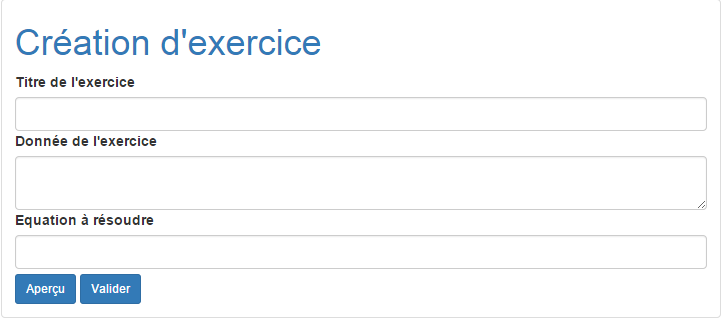
\includegraphics{create.png}

Tout est dit, il suffit juste de spécifier le titre, la donnée ainsi que l'équation à résoudre pour pouvoir créer un exercice. Si vous observez bien, vous remarquez un bouton aperçu présent
à côté de celui nommé valider. Celui-ci , sert une fois avoir insérer les données voulu d'avoir un aperçu de ce qui sera présent dans l'exercice.


\section{Le code permettant la création}
\label{create:le-code-permettant-la-creation}

\subsection{Le template}
\label{create:le-template}
Dans le template exercises/templates/create.html, rien de spécial y apparait mise à part les 2 \textless{}input\textgreater{} et le \textless{}textarea\textgreater{} qui seront utilisés dans la vue ``create'' plus tard.

\begin{Verbatim}[commandchars=\\\{\}]
\PYG{n+nt}{\PYGZlt{}input} \PYG{n+na}{type=}\PYG{l+s}{\PYGZdq{}text\PYGZdq{}} \PYG{n+na}{id=}\PYG{l+s}{\PYGZdq{}title\PYGZdq{}} \PYG{n+na}{name=}\PYG{l+s}{\PYGZdq{}title\PYGZdq{}} \PYG{n+na}{class=}\PYG{l+s}{\PYGZdq{}form\PYGZhy{}control\PYGZdq{}}\PYG{n+nt}{\PYGZgt{}}
\PYG{n+nt}{\PYGZlt{}textarea} \PYG{n+na}{id=}\PYG{l+s}{\PYGZdq{}donnee\PYGZdq{}} \PYG{n+na}{class=}\PYG{l+s}{\PYGZdq{}form\PYGZhy{}control\PYGZdq{}} \PYG{n+na}{name=}\PYG{l+s}{\PYGZdq{}donnee\PYGZdq{}}\PYG{n+nt}{\PYGZgt{}}\PYG{n+nt}{\PYGZlt{}/textarea\PYGZgt{}}
\PYG{n+nt}{\PYGZlt{}input} \PYG{n+na}{type=}\PYG{l+s}{\PYGZdq{}text\PYGZdq{}} \PYG{n+na}{id=}\PYG{l+s}{\PYGZdq{}equation\PYGZdq{}} \PYG{n+na}{name=}\PYG{l+s}{\PYGZdq{}equation\PYGZdq{}} \PYG{n+na}{class=}\PYG{l+s}{\PYGZdq{}form\PYGZhy{}control\PYGZdq{}}\PYG{n+nt}{\PYGZgt{}}
\end{Verbatim}

Il est à ajouter que pour le bouton aperçu, un code javascript a été nécéssaire.

Le voici:

\begin{Verbatim}[commandchars=\\\{\}]
\PYG{n+nx}{\PYGZdl{}}\PYG{p}{(}\PYG{n+nb}{document}\PYG{p}{)}\PYG{p}{.}\PYG{n+nx}{ready}\PYG{p}{(}\PYG{k+kd}{function}\PYG{p}{(}\PYG{p}{)} \PYG{p}{\PYGZob{}}
    \PYG{n+nx}{\PYGZdl{}}\PYG{p}{(}\PYG{l+s+s2}{\PYGZdq{}\PYGZsh{}voir\PYGZdq{}}\PYG{p}{)}\PYG{p}{.}\PYG{n+nx}{click}\PYG{p}{(}\PYG{k+kd}{function}\PYG{p}{(}\PYG{p}{)} \PYG{p}{\PYGZob{}}
        \PYG{k+kd}{var} \PYG{n+nx}{formule} \PYG{o}{=} \PYG{n+nx}{\PYGZdl{}}\PYG{p}{(}\PYG{l+s+s2}{\PYGZdq{}\PYGZsh{}equation\PYGZdq{}}\PYG{p}{)}\PYG{p}{.}\PYG{n+nx}{val}\PYG{p}{(}\PYG{p}{)}\PYG{p}{;}
        \PYG{k+kd}{var} \PYG{n+nx}{donnee}\PYG{o}{=} \PYG{n+nx}{\PYGZdl{}}\PYG{p}{(}\PYG{l+s+s2}{\PYGZdq{}\PYGZsh{}donnee\PYGZdq{}}\PYG{p}{)}\PYG{p}{.}\PYG{n+nx}{val}\PYG{p}{(}\PYG{p}{)}\PYG{p}{;}
        \PYG{n+nx}{\PYGZdl{}}\PYG{p}{(}\PYG{l+s+s2}{\PYGZdq{}\PYGZsh{}formule\PYGZdq{}}\PYG{p}{)}\PYG{p}{.}\PYG{n+nx}{text}\PYG{p}{(}\PYG{n+nx}{formule}\PYG{p}{)}\PYG{p}{;}
        \PYG{n+nx}{\PYGZdl{}}\PYG{p}{(}\PYG{l+s+s2}{\PYGZdq{}\PYGZsh{}donnee\PYGZhy{}apercu\PYGZdq{}}\PYG{p}{)}\PYG{p}{.}\PYG{n+nx}{text}\PYG{p}{(}\PYG{n+nx}{donnee}\PYG{p}{)}
        \PYG{n+nx}{\PYGZdl{}}\PYG{p}{(}\PYG{l+s+s2}{\PYGZdq{}\PYGZsh{}apercu\PYGZdq{}}\PYG{p}{)}\PYG{p}{.}\PYG{n+nx}{css}\PYG{p}{(}\PYG{p}{\PYGZob{}}\PYG{n+nx}{display} \PYG{o}{:} \PYG{l+s+s2}{\PYGZdq{}block\PYGZdq{}}\PYG{p}{\PYGZcb{}}\PYG{p}{)}
    \PYG{p}{\PYGZcb{}}\PYG{p}{)}
\PYG{p}{\PYGZcb{}}\PYG{p}{)}\PYG{p}{;}
\end{Verbatim}

Jquery permet de faire une modification du DOM beaucoup plus rapide que du javascript simple.


\subsection{La vue}
\label{create:la-vue}
Pour ce qui est du code fonctionnant derrière cette partie de mon application, la difficulté se trouve surtout dans la sauvegarde des données.

En effet, il a fallu que pour chaques balises \textless{}textarea\textgreater{} ou \textless{}input\textgreater{} permettant d'entrer les valeurs du titre, de la donnée et de l'équation puissent être enregistrer dans une variable et les enregistrer
dans la base de donnée dans la table ``Exercices''. Le code qui m'a permis de faire cela se trouve dans le fichier views.py dans la vue ``create''.

\begin{Verbatim}[commandchars=\\\{\}]
\PYG{k}{def} \PYG{n+nf}{create}\PYG{p}{(}\PYG{n}{request}\PYG{p}{)}\PYG{p}{:}
\PYG{k}{if} \PYG{n}{request}\PYG{o}{.}\PYG{n}{method} \PYG{o}{==} \PYG{l+s}{\PYGZsq{}}\PYG{l+s}{POST}\PYG{l+s}{\PYGZsq{}}\PYG{p}{:} \PYG{c}{\PYGZsh{} sauvegarde des données dans la db}
    \PYG{n}{title} \PYG{o}{=} \PYG{n}{request}\PYG{o}{.}\PYG{n}{POST}\PYG{p}{[}\PYG{l+s}{\PYGZsq{}}\PYG{l+s}{title}\PYG{l+s}{\PYGZsq{}}\PYG{p}{]}
    \PYG{n}{donnee} \PYG{o}{=} \PYG{n}{request}\PYG{o}{.}\PYG{n}{POST}\PYG{p}{[}\PYG{l+s}{\PYGZsq{}}\PYG{l+s}{donnee}\PYG{l+s}{\PYGZsq{}}\PYG{p}{]}
    \PYG{n}{equation} \PYG{o}{=} \PYG{n}{request}\PYG{o}{.}\PYG{n}{POST}\PYG{p}{[}\PYG{l+s}{\PYGZsq{}}\PYG{l+s}{equation}\PYG{l+s}{\PYGZsq{}}\PYG{p}{]}

    \PYG{n}{Exercise}\PYG{p}{(}\PYG{n}{title}\PYG{o}{=}\PYG{n}{title}\PYG{p}{,} \PYG{n}{donnee}\PYG{o}{=}\PYG{n}{donnee}\PYG{p}{,} \PYG{n}{equation}\PYG{o}{=}\PYG{n}{equation}\PYG{p}{)}\PYG{o}{.}\PYG{n}{save}\PYG{p}{(}\PYG{p}{)}

    \PYG{k}{return} \PYG{n}{HttpResponseRedirect}\PYG{p}{(}\PYG{n}{reverse}\PYG{p}{(}\PYG{l+s}{\PYGZdq{}}\PYG{l+s}{exercises:index}\PYG{l+s}{\PYGZdq{}}\PYG{p}{)}\PYG{p}{)}
\PYG{k}{else}\PYG{p}{:}
    \PYG{k}{return} \PYG{n}{render}\PYG{p}{(}\PYG{n}{request}\PYG{p}{,} \PYG{l+s}{\PYGZsq{}}\PYG{l+s}{exercises/create.html}\PYG{l+s}{\PYGZsq{}}\PYG{p}{)}
\end{Verbatim}

La partie se trouvant dans le ``if'' permet de mettre dans des variables les valeurs récupérées. Il est a noté qu'il y a une partie else présente dans cette vue.
Cela indique seulement que si il n'y a pas de données à enregistrer, le template se charge normalement. Dès le moment où des données sont enregistrées, l'utilisateur est renvoyé à la page d'accueil.
Ceci permet juste que l'utilisateur ne crée pas de doublons en cliquant plusieurs fois sur ``Valider'' et qu'il comprenne que son exercice a bien été enregistré.


\chapter{Comment, où résoudre un exercice?}
\label{find:comment-ou-resoudre-un-exercice}\label{find::doc}

\section{La page de résolution d'exercice}
\label{find:la-page-de-resolution-d-exercice}
L'application exercice possède un onglet \href{https://webmath-thirteenfoil8.c9.io/exercises/find/}{Résoudre un exercice} , présent sur le menu latéral permettant de renvoyer à la page de
résolution d'exercice.

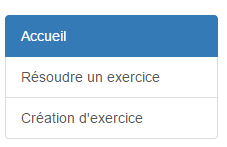
\includegraphics{onglet.png}

Cliquez sur l'onglet Résoudre un exercice pour aller sur la page de résolution. Une fois sur la page, une liste ressemblant à ça devrait apparaître:

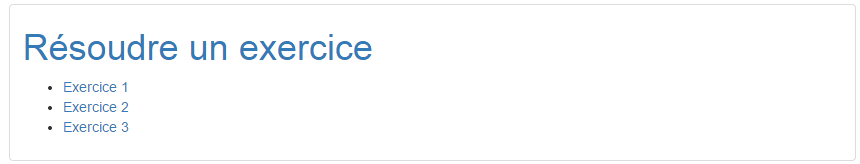
\includegraphics{find.png}

Comme vous pouvez le constater, tous les exercices créés sont présents sur cette page. Il suffit juste de cliquer sur l'exercice dont vous avez besoin pour être redirigé vers celui-ci.


\section{Le code permettant la résolution :}
\label{find:le-code-permettant-la-resolution}

\subsection{Les templates}
\label{find:les-templates}

\subsubsection{Le template find.html}
\label{find:le-template-find-html}
Le template de cette page se trouve sous le fichier exercises/templates/find.html . Dans celui-ci, il y a une chose notable qui mérite d'être expliqué c'est la récupération d'urls des exercices.

\begin{Verbatim}[commandchars=\\\{\}]
\PYG{n+nt}{\PYGZlt{}ul}\PYG{n+nt}{\PYGZgt{}}
    \PYGZob{}\PYGZpc{} for exercise in exercises\PYGZus{}list \PYGZpc{}\PYGZcb{}
        \PYG{n+nt}{\PYGZlt{}li}\PYG{n+nt}{\PYGZgt{}}\PYG{n+nt}{\PYGZlt{}a} \PYG{n+na}{href=}\PYG{l+s}{\PYGZdq{}\PYGZob{}\PYGZpc{} url \PYGZsq{}exercises:resolve\PYGZsq{} exercise.id \PYGZpc{}\PYGZcb{}\PYGZdq{}}\PYG{n+nt}{\PYGZgt{}}\PYGZob{}\PYGZob{} exercise.title \PYGZcb{}\PYGZcb{}\PYG{n+nt}{\PYGZlt{}/a\PYGZgt{}}\PYG{n+nt}{\PYGZlt{}/li\PYGZgt{}}
    \PYGZob{}\PYGZpc{} endfor \PYGZpc{}\PYGZcb{}
\PYG{n+nt}{\PYGZlt{}/ul\PYGZgt{}}
\end{Verbatim}

Nous verrons par la suite d'où vient la liste '' exercises\_list''. Mais cette liste permet de créer une liste html avec tous les exercices présents dans la base de données et de faire un lien
permettant d'accéder à leur page


\subsubsection{Le template resolve.html}
\label{find:le-template-resolve-html}
Le template resolve.html est le template où apparaissent tous les exercices qui ont été créés par les professeurs. Chaque exercice possède une page et pour chaque nouveau exercice, une nouvelle page
est créée. Ceci permet aux exercices de ne pas dépendre les uns des autres et d'être totalement indépendants.

Nous pouvons faire resortir l'appel des éléments de chaque objet appartenant à ``Exercises'' en les utilisant dans de simples balises html.

\begin{Verbatim}[commandchars=\\\{\}]
\PYG{n+nt}{\PYGZlt{}h1} \PYG{n+na}{id=}\PYG{l+s}{\PYGZdq{}title\PYGZdq{}}\PYG{n+nt}{\PYGZgt{}}\PYGZob{}\PYGZob{} exercise.title \PYGZcb{}\PYGZcb{}\PYG{n+nt}{\PYGZlt{}/h1\PYGZgt{}}
\PYG{n+nt}{\PYGZlt{}div} \PYG{n+na}{class=}\PYG{l+s}{\PYGZdq{}thumbnail\PYGZdq{}}\PYG{n+nt}{\PYGZgt{}}
    \PYG{n+nt}{\PYGZlt{}p} \PYG{n+na}{id =}\PYG{l+s}{\PYGZdq{}donnee\PYGZdq{}}\PYG{n+nt}{\PYGZgt{}}\PYGZob{}\PYGZob{} exercise.donnee \PYGZcb{}\PYGZcb{}\PYG{n+nt}{\PYGZlt{}/p\PYGZgt{}}
    \PYG{n+nt}{\PYGZlt{}p}\PYG{n+nt}{\PYGZgt{}}\PYGZob{}\PYGZob{} exercise.equation \PYGZcb{}\PYGZcb{}\PYG{n+nt}{\PYGZlt{}/p\PYGZgt{}}
    \PYG{n+nt}{\PYGZlt{}h6}\PYG{n+nt}{\PYGZgt{}}crée le :\PYGZob{}\PYGZob{} exercise.created\PYGZus{}on  \PYGZcb{}\PYGZcb{}\PYG{n+nt}{\PYGZlt{}/h6\PYGZgt{}}
    \PYG{n+nt}{\PYGZlt{}input} \PYG{n+na}{type=}\PYG{l+s}{\PYGZdq{}text\PYGZdq{}} \PYG{n+na}{id=}\PYG{l+s}{\PYGZdq{}equation\PYGZdq{}} \PYG{n+na}{name=}\PYG{l+s}{\PYGZdq{}equation\PYGZdq{}} \PYG{n+na}{class=}\PYG{l+s}{\PYGZdq{}form\PYGZhy{}control\PYGZdq{}}\PYG{n+nt}{\PYGZgt{}}
\PYG{n+nt}{\PYGZlt{}/div\PYGZgt{}}
\end{Verbatim}


\subsection{Les vues}
\label{find:les-vues}

\subsubsection{La vue find}
\label{find:la-vue-find}
La vue find se trouvant dans le fichier views.py est la vue qui nous permet de récupérer tous les exercices présent dans la base de données. Cette vue est importante car sans elle, le seul moyen
d'accéder aux exercices serait de connaître l'url de ceux-ci et de les écrire à la main. Tandis que là, il suffit de se rendre sur la page \href{https://webmath-thirteenfoil8.c9.io/exercises/find/}{Résoudre un exercice}
pour voir tous les exercices qui ont été créés. Cela est très pratique notamment si un élève veut pouvoir s'entraîner sur plusieurs matières ou si tout simplement il a envie de faire quelques exercices
de manière aléatoire.

Le code de cette vue est le suivant :

\begin{Verbatim}[commandchars=\\\{\}]
\PYG{k}{def} \PYG{n+nf}{find}\PYG{p}{(}\PYG{n}{request}\PYG{p}{)}\PYG{p}{:}
\PYG{n}{latest\PYGZus{}exercise\PYGZus{}list} \PYG{o}{=} \PYG{n}{Exercise}\PYG{o}{.}\PYG{n}{objects}\PYG{o}{.}\PYG{n}{all}\PYG{p}{(}\PYG{p}{)}
\PYG{k}{return} \PYG{n}{render}\PYG{p}{(}\PYG{n}{request}\PYG{p}{,} \PYG{l+s}{\PYGZsq{}}\PYG{l+s}{exercises/find.html}\PYG{l+s}{\PYGZsq{}}\PYG{p}{,} \PYG{p}{\PYGZob{}}\PYG{l+s}{\PYGZdq{}}\PYG{l+s}{exercises\PYGZus{}list}\PYG{l+s}{\PYGZdq{}} \PYG{p}{:} \PYG{n}{latest\PYGZus{}exercise\PYGZus{}list}\PYG{p}{\PYGZcb{}}\PYG{p}{)}
\end{Verbatim}

La fonction objects.all() permet de récuperer tous les exercices présents dans la table Exercises. Il suffit de faire une boucle ``for'' dans le template pour les afficher.


\subsubsection{La vue resolve}
\label{find:la-vue-resolve}
La vue resolve se trouvant dans le fichier views.py est la vue qui nous permet d'afficher un exercice dans son template resolve.html et si il n'y a pas d'exercice suite à l'url entré par l'utilisateur,
elle renvoit une erreur 404. Grâce à celle-ci, chaque exercice à sa propre page.

Le code de cette vue est assez rudimentaire mais l'import ainsi que l'utilisation de ``get\_object\_or\_404'' est à noter.

\begin{Verbatim}[commandchars=\\\{\}]
\PYG{k+kn}{from} \PYG{n+nn}{django.shortcuts} \PYG{k+kn}{import} \PYG{n}{get\PYGZus{}object\PYGZus{}or\PYGZus{}404}

\PYG{k}{def} \PYG{n+nf}{resolve}\PYG{p}{(}\PYG{n}{request}\PYG{p}{,} \PYG{n}{n\PYGZus{}exercise}\PYG{p}{)}\PYG{p}{:}
\PYG{n}{exercise} \PYG{o}{=} \PYG{n}{get\PYGZus{}object\PYGZus{}or\PYGZus{}404}\PYG{p}{(}\PYG{n}{Exercise}\PYG{p}{,} \PYG{n+nb}{id}\PYG{o}{=}\PYG{n}{n\PYGZus{}exercise}\PYG{p}{)}
\PYG{k}{return} \PYG{n}{render}\PYG{p}{(}\PYG{n}{request}\PYG{p}{,} \PYG{l+s}{\PYGZsq{}}\PYG{l+s}{exercises/resolve.html}\PYG{l+s}{\PYGZsq{}}\PYG{p}{,} \PYG{p}{\PYGZob{}}\PYG{l+s}{\PYGZdq{}}\PYG{l+s}{exercise}\PYG{l+s}{\PYGZdq{}} \PYG{p}{:} \PYG{n}{exercise}\PYG{p}{\PYGZcb{}}\PYG{p}{)}
\end{Verbatim}


\chapter{Indices and tables}
\label{index:indices-and-tables}\begin{itemize}
\item {} 
\emph{genindex}

\item {} 
\emph{modindex}

\item {} 
\emph{search}

\end{itemize}



\renewcommand{\indexname}{Index}
\printindex
\end{document}
